%2multibyte Version: 5.50.0.2960 CodePage: 1252

\documentclass[notes=show,handout]{beamer}\usepackage[]{graphicx}\usepackage[]{color}
% maxwidth is the original width if it is less than linewidth
% otherwise use linewidth (to make sure the graphics do not exceed the margin)
\makeatletter
\def\maxwidth{ %
  \ifdim\Gin@nat@width>\linewidth
    \linewidth
  \else
    \Gin@nat@width
  \fi
}
\makeatother

\definecolor{fgcolor}{rgb}{0.345, 0.345, 0.345}
\newcommand{\hlnum}[1]{\textcolor[rgb]{0.686,0.059,0.569}{#1}}%
\newcommand{\hlstr}[1]{\textcolor[rgb]{0.192,0.494,0.8}{#1}}%
\newcommand{\hlcom}[1]{\textcolor[rgb]{0.678,0.584,0.686}{\textit{#1}}}%
\newcommand{\hlopt}[1]{\textcolor[rgb]{0,0,0}{#1}}%
\newcommand{\hlstd}[1]{\textcolor[rgb]{0.345,0.345,0.345}{#1}}%
\newcommand{\hlkwa}[1]{\textcolor[rgb]{0.161,0.373,0.58}{\textbf{#1}}}%
\newcommand{\hlkwb}[1]{\textcolor[rgb]{0.69,0.353,0.396}{#1}}%
\newcommand{\hlkwc}[1]{\textcolor[rgb]{0.333,0.667,0.333}{#1}}%
\newcommand{\hlkwd}[1]{\textcolor[rgb]{0.737,0.353,0.396}{\textbf{#1}}}%
\let\hlipl\hlkwb

\usepackage{framed}
\makeatletter
\newenvironment{kframe}{%
 \def\at@end@of@kframe{}%
 \ifinner\ifhmode%
  \def\at@end@of@kframe{\end{minipage}}%
  \begin{minipage}{\columnwidth}%
 \fi\fi%
 \def\FrameCommand##1{\hskip\@totalleftmargin \hskip-\fboxsep
 \colorbox{shadecolor}{##1}\hskip-\fboxsep
     % There is no \\@totalrightmargin, so:
     \hskip-\linewidth \hskip-\@totalleftmargin \hskip\columnwidth}%
 \MakeFramed {\advance\hsize-\width
   \@totalleftmargin\z@ \linewidth\hsize
   \@setminipage}}%
 {\par\unskip\endMakeFramed%
 \at@end@of@kframe}
\makeatother

\definecolor{shadecolor}{rgb}{.97, .97, .97}
\definecolor{messagecolor}{rgb}{0, 0, 0}
\definecolor{warningcolor}{rgb}{1, 0, 1}
\definecolor{errorcolor}{rgb}{1, 0, 0}
\newenvironment{knitrout}{}{} % an empty environment to be redefined in TeX

\usepackage{alltt}
%%%%%%%%%%%%%%%%%%%%%%%%%%%%%%%%%%%%%%%%%%%%%%%%%%%%%%%%%%%%%%%%%%%%%%%%%%%%%%%%%%%%%%%%%%%%%%%%%%%%%%%%%%%%%%%%%%%%%%%%%%%%%%%%%%%%%%%%%%%%%%%%%%%%%%%%%%%%%%%%%%%%%%%%%%%%%%%%%%%%%%%%%%%%%%%%%%%%%%%%%%%%%%%%%%%%%%%%%%%%%%%%%%%%%%%%%%%%%%%%%%%%%%%%%%%%
\usepackage{amsfonts}
\usepackage{amsmath}
\usepackage{graphicx}
\usepackage{mathpazo}
\usepackage{hyperref}
\usepackage{multimedia}

\setcounter{MaxMatrixCols}{10}

\newenvironment{stepenumerate}{\begin{enumerate}[<+->]}{\end{enumerate}}
\newenvironment{stepitemize}{\begin{itemize}[<+->]}{\end{itemize} }
\newenvironment{stepenumeratewithalert}{\begin{enumerate}[<+-| alert@+>]}{\end{enumerate}}
\newenvironment{stepitemizewithalert}{\begin{itemize}[<+-| alert@+>]}{\end{itemize} }
\usetheme{Madrid}

\setcounter{MaxMatrixCols}{10}
\newtheorem{remark}{Remark}[section]
\newtheorem{proposition}{Proposition}[section]
\newtheorem{interpretation}{Interpretation}[section]
\newtheorem{goal}{Goal}[section]
\newtheorem{statement}{Statement}[section]
\newtheorem{aes}{Aim \& Scope}[section]
\newtheorem{exercise}{Exercise}[section]
\renewcommand{\Pr}{P}


%%%%%%%%%%%%%%%%%%%%%%%%%%%%%%%%%%%%%%%%%%%%%%%%%%%%%%%%%%%%%%%%%%%%%%%%%%%%%%%
% GSEM COLORS
%%%%%%%%%%%%%%%%%%%%%%%%%%%%%%%%%%%%%%%%%%%%%%%%%%%%%%%%%%%%%%%%%%%%%%%%%%%%%%%
\definecolor{darkGSEM}{RGB}{70,95,127}
\definecolor{darkGSEM2}{RGB}{40,80,150}
\definecolor{GSEM}{RGB}{96,121,153} % GSEM 10% lighter

%%% Global colors
\setbeamercolor*{palette primary}{use=structure,fg=white,bg=darkGSEM}
\setbeamercolor*{palette quaternary}{use=structure,fg=white,bg=darkGSEM!90}
\setbeamercolor{frametitle}{fg=white,bg=GSEM!80}

%%% TOC colors
\setbeamercolor{section in toc}{fg=darkGSEM}

%%% itemize colors
\setbeamertemplate{itemize items}[circle]
\setbeamercolor{itemize item}{fg=darkGSEM2}
\setbeamercolor{itemize subitem}{fg=darkGSEM2}
\setbeamercolor{itemize subsubitem}{fg=darkGSEM2}


%%% enumerate colors
\setbeamercolor{item projected}{fg=white,bg=GSEM}
\setbeamertemplate{enumerate item}{\insertenumlabel.}
\setbeamercolor{enumerate item}{fg=darkGSEM2}
\setbeamercolor{enumerate subitem}{fg=darkGSEM2}
\setbeamercolor{enumerate subsubitem}{fg=darkGSEM2}


\AtBeginSection[]
{
  \begin{frame}
    \frametitle{Outline}
    \tableofcontents[currentsection]
  \end{frame}
}

%%%%%%%%%%%%%%%%%%%%%%%%%%%%%%%%%%%%%%%%%%%%%%%%%%%%%%%%%%%%%%%%%%%%%%%%%%%%%%%%
\IfFileExists{upquote.sty}{\usepackage{upquote}}{}
\begin{document}


\title[S110015]{Probability 1}
\subtitle{Lecture 10: Bivariate Discrete Random Variables}
\author[Flores-Agreda, La Vecchia]{Dr. Daniel Flores-Agreda, \\[0.5em] \tiny{(based on the notes of Prof. Davide La Vecchia)}}
\date{Spring Semester 2021}


\begin{frame}
  \titlepage
\end{frame}

\begin{frame}{Objectives}
  \begin{itemize}
  \item Introduce the Notion of Joint PMF's for discrete RV and the main implications \bigskip
  \begin{itemize}
  \item Difference between Conditional and Marginal PMF \bigskip
  \item Joint and Conditional Expectations \bigskip
  \item Covariance and Correlation \bigskip
  \end{itemize}
  \end{itemize}
\end{frame}

%TCIMACRO{\TeXButton{BeginFrame}{\begin{frame}}}%
%BeginExpansion
%\begin{frame}%
%%EndExpansion
%
%%\subsection{Jointly distributed discrete random variables}
%
%%%TCIMACRO{\TeXButton{BeginFrame}{\begin{frame}}}%
%%%BeginExpansion
%%\begin{frame}%
%%%EndExpansion
%%
%\frametitle{Jointly distributed discrete random variables}
%%
%\begin{example}
%\begin{stepitemize}
%\item Two production lines manufacture a certain type of item.
%
%\item Suppose that the capacity (on any given day) is 5 items for \emph{Line
%I }and 3 items for \emph{Line II}.
%
%\item Assume that the number of items actually produced by either production
%line is a random variable.
%
%\item Let $(X,Y)$ represent the 2-dimensional random variable yielding the
%number of items produced by \emph{Line I} and \emph{Line II}, respectively.
%
%\item The joint probability (mass) function is
%$$
%\Pr(\{X=x \quad \text{and} \quad Y=y\})
%$$
%for all possible values $x$ and $y$
%\end{stepitemize}
%\end{example}
%\end{frame}%
%
%
%\begin{frame}
%\frametitle{Jointly distributed discrete random variables}
%\begin{example}[cont'd]
%\begin{tabular}{|cc||c|c|c|c|c|c||c|}
%\hline
%& $x$ & $0$ & $1$ & $2$ & $3$ & $4$ & $5$ & $\Pr \left\{ Y=y\right\} $ \\
%$y$ &  &  &  &  &  &  &  &  \\ \hline\hline
%$0$ &  & $0$ & $0.01$ & $0.03$ & $0.05$ & $0.07$ & $0.09$ & $0.25$ \\ \hline
%$1$ &  & $0.01$ & $0.02$ & $0.04$ & $0.05$ & $0.06$ & $0.08$ & $0.26$ \\
%\hline
%$2$ &  & $0.01$ & $0.03$ & $0.05$ & $0.05$ & $0.05$ & $0.06$ & $0.25$ \\
%\hline
%$3$ &  & $0.01$ & $0.02$ & $0.04$ & $0.06$ & $0.06$ & $0.05$ & $0.24$ \\
%\hline\hline
%$\Pr \left\{ X=x\right\} $ &  & $0.03$ & $0.08$ & $0.16$ & $0.21$ & $0.24$ &
%$0.28$ & $1$ \\ \hline
%\end{tabular}
%\end{example}
%\end{frame}%

%%%%%%%%%%%%%%%%%%%%%%%%%%%%%%%%%%%%%%%%%%%%%%%%%%%%%%%%%%%%%%%%%%%%%%%%%%%%%%%
\section{Joint Probability Functions}
%%%%%%%%%%%%%%%%%%%%%%%%%%%%%%%%%%%%%%%%%%%%%%%%%%%%%%%%%%%%%%%%%%%%%%%%%%%%%%%

\begin{frame}{\secname}

  \begin{definition}[Joint Probability Mass Function]
  Let $X$ and $Y$ be a pair of discrete random variables

  \medskip

  Their  \textbf{Joint Probability Mass Function (Joint PMF)} expresses the probability that $X$ takes on a specific
  value $x$ and $Y$ takes on the specific value $y$ \textbf{simultaneously}.


  \begin{equation*}
  p_{X,Y}\left( x,y\right) =\Pr (\left\{ X=x\cap Y=y\right\})
  \end{equation*}
  thought of as a \textbf{function} of $x$ and $y$.
  \end{definition}

\end{frame}

\begin{frame}{\secname}

  The joint PMF has two essential properties:

  \medskip

  \begin{enumerate}
  \item The value of the Joint PMF is always non-negative
  $$p_{X,Y}\left( x,y\right) \geq 0 \text{\ for all possible pairs \ }
  \left(x,y\right)$$

  \item The sum over all combinations of $x$ and $y$ values is equal to one
  $$\sum_{x}\sum_{y}\Pr ( \left\{ X=x\cap Y=y\right\}) =1$$
  \end{enumerate}

\end{frame}


\begin{frame}{\secname}

  \begin{definition}[Marginal Probability Mass Functions]
  The Probability Mass Function (PMF) of the \emph{discrete} random variable
  $X$ is called its \emph{Marginal} PMF.

  It can be obtained by summing the joint probabilities relating to pairs $
  (X,Y)$ over \textbf{all possible values of $Y$}:
  \begin{equation*}
  p_{X}(x)=\sum_{y}p_{X,Y}(x,y).
  \end{equation*}
  \end{definition}

  Equivalently, the Marginal PMF of $Y$ can be obtained by summing the joint probabilities relating to pairs $(X,Y)$ over \textbf{all possible values of $X$}:
  \begin{equation*}
  p_{Y}(y)=\sum_{x}p_{X,Y}(x,y).
  \end{equation*}

\end{frame}


\begin{frame}{\secname}


  \begin{example}[Caplets]
  \begin{footnotesize}

  \begin{itemize}
  \item Two caplets are selected at random from a bottle containing \textbf{3
  aspirins}, \textbf{2 sedatives} and \textbf{2 placebo} caplets.

  \item We are assuming that the caplets are well mixed and that each has an
  equal chance of being selected.

  \item Let $X$ and $Y$ denote:
  \begin{itemize}
  \item $X$ : the numbers of aspirin caplets,
  \item $Y$ : the number of sedative caplets,
  \end{itemize}
  that we pick when we draw when we draw two caplets from the bottle.
  %
  %\item We want to find the probabilities associated with all possible values
  %of $X$ and $Y$.
  %
  %\item All the possible pairs of $(X,Y)$ are $(0,0)$,$(1,0)$, $(0,1)$, $(1,1)$%
  %, $(2,0)$, and $(0,2)$.
  \end{itemize}
  \end{footnotesize}
  \end{example}
\end{frame}


\begin{frame}{\secname}
  \begin{example}[Caplets]
  \begin{footnotesize}

  Number of sets of 2 caplets out of 7:

  $${7 \choose 2} = \frac{7!}{2!\times (7-2)!} = \frac{7!}{2! \times 5!} = \frac{6\times 7}{2} = 3\times 7 = 21$$

  \end{footnotesize}
  \end{example}
\end{frame}


\begin{frame}{\secname}
  \begin{example}[continued]
  \begin{footnotesize}

  The Joint Probabilities can be found with Combinatorial Formulae:

  \begin{itemize}
  \item $p_{X,Y}(0, 0) = {3 \choose 0}{2 \choose 0}{2 \choose 2} \left/ 21 \right. = 1/21$
  \item $p_{X,Y}(1, 0) = {3 \choose 1}{2 \choose 0}{2 \choose 1} \left/ 21 \right. = 6/21$
  \item $p_{X,Y}(2, 0) = {3 \choose 2}{2 \choose 0}{2 \choose 0} \left/ 21 \right. = 3/21$
  \item $p_{X,Y}(0, 1) = {3 \choose 0}{2 \choose 1}{2 \choose 1} \left/ 21 \right. = 4/21$
  \item $p_{X,Y}(1, 1) = {3 \choose 1}{2 \choose 1}{2 \choose 0} \left/ 21 \right. = 6/21$
  \item $p_{X,Y}(2, 1) = 0$ since $2+1 = 3 > 2$
  \item $p_{X,Y}(0, 2) = {3 \choose 0}{2 \choose 2}{2 \choose 0} \left/ 21 \right. = 1/21$
  \item $p_{X,Y}(1, 2) = 0$ since $1+2 = 3 > 2$
  \item $p_{X,Y}(2, 2) = 0$ since $2+2 = 4 > 2$
  \end{itemize}

  \end{footnotesize}
  \end{example}
\end{frame}


%\begin{frame}{\secname}%
%%EndExpansion
%
%\frametitle{First Example}
%
%%\begin{example}[cont'd]
%\begin{stepitemize}
%\item To work out each of these probabilties, we use combinations.
%
%\begin{stepitemize}
%\item e.g., the outcome $(1,1)$ corresponds to choosing only one asprin
%caplet and only one sedative caplet.
%
%\begin{stepitemize}
%\item But that one asprin caplet could be any one of the three available in
%the jar,
%
%\item and that one sedative caplet could be either one of the two available
%in the jar.
%
%\item So the number of possible combinations that satisfy $\left( x,y\right)
%=(1,1)$ are%
%\begin{eqnarray*}
%\underset{\text{\# asprin}}{\underbrace{\left(
%\begin{array}{c}
%3 \\
%1%
%\end{array}%
%\right) }}\times \underset{\text{\# sedative}}{\underbrace{\left(
%\begin{array}{c}
%2 \\
%1%
%\end{array}%
%\right) }}\times \underset{\text{\# placebo}}{\underbrace{\left(
%\begin{array}{c}
%2 \\
%0%
%\end{array}%
%\right) }} &=&\frac{3!}{1!2!}\times \frac{2!}{1!1!}\times \frac{2!}{2!0!} \\
%&=&3\times 2\times 1=6
%\end{eqnarray*}
%\end{stepitemize}
%
%\item We can work out the number of possible combinations for the remaining $%
%\left( x,y\right) $ pairs similarly.
%\end{stepitemize}
%\end{stepitemize}
%%\end{example}
%%TCIMACRO{\TeXButton{EndFrame}{\end{frame}}}%
%%BeginExpansion
%\end{frame}%
%%EndExpansion
%%
%%%%TCIMACRO{\TeXButton{BeginFrame}{\begin{frame}{\secname}}}%
%%%BeginExpansion
%\begin{frame}{\secname}%
%%EndExpansion
%
%\frametitle{First Example (Discrete)}
%
%The \emph{probability} can be tabulated as
%
%\begin{center}
%\begin{tabular}{|c||c||c||c|}
%\hline
%${\small (x,y)}$ & {\small event drawn} & {\small combinations} & $\Pr
%\left\{ \left( X,Y\right) =\left( x,y\right) \right\} $ \\ \hline\hline
%${\small (0,0)}$ & {\small 2 placebos} & ${\small 1}$ & ${\small 1/21}$ \\
%\hline
%${\small (1,0)}$ & {\small 1 asprin,1 placebo} & ${\small 6}$ & ${\small 6/21%
%}$ \\ \hline
%${\small (0,1)}$ & {\small 1 sedative, 1 placebo} & ${\small 4}$ & ${\small %
%4/21}$ \\ \hline
%${\small (1,1)}$ & {\small 1 asprin, 1 placebo} & ${\small 6}$ & ${\small %
%6/21}$ \\ \hline
%${\small (2,0)}$ & {\small 2 asprin} & ${\small 3}$ & ${\small 3/21}$ \\
%\hline
%${\small (0,2)}$ & {\small 2 sedatives} & ${\small 1}$ & ${\small 1/21}$ \\
%\hline\hline
%{\small Total} &  & ${\small 21}$ & ${\small 1}$ \\ \hline
%\end{tabular}
%\end{center}
%
%TCIMACRO{\TeXButton{EndFrame}{\end{frame}}}%
%BeginExpansion
%\end{frame}%
%%EndExpansion
%
%%TCIMACRO{\TeXButton{BeginFrame}{\begin{frame}{\secname}}}%
%%BeginExpansion

\begin{frame}{\secname}
\begin{example}
  \begin{footnotesize}
Notice that we can infer the following Joint PMF:
  $$P(X=x \cap Y=y) = p(x, y) = \left\{ \begin{array}{ll}
  {3 \choose x}{2 \choose y}{2 \choose 2-x-y} \left/{7 \choose 2}\right. & x+y\leq 2\\
  0 &otherwise\end{array}\right.$$
  \end{footnotesize}
\end{example}
\end{frame}

\begin{frame}{\secname}
  \begin{example}[continued]
  \begin{footnotesize}
  Tabulating the \underline{\emph{joint}} probabilities as follows,
  we can easily work out the \underline{\emph{marginal}}
  probabilities

  \begin{center}
  $%
  \begin{tabular}{|cc||c|c|c||c|}
  \hline
  & $x$ & $0$ & $1$ & $2$ & $\Pr \left\{ Y=y\right\} $ \\
  $y$ &  &  &  &  &  \\ \hline\hline
  $0$ &  & $1/21$ & $6/21$ & $3/21$ & $10/21$ \\ \hline
  $1$ &  & $4/21$ & $6/21$ & $0$ & $10/21$ \\ \hline
  $2$ &  & $1/21$ & $0$ & $0$ & $1/21$ \\ \hline\hline
  $\Pr \left\{ X=x\right\} $ &  & $6/21$ & $12/21$ & $3/21$ & $1$ \\ \hline
  \end{tabular}%
  $
  \end{center}
  \end{footnotesize}
  \end{example}
  %\begin{stepitemize}
  %\item Note that the expected value for $X$ and $Y$ are, respectively,
  %
  %\begin{stepitemize}
  %\item $E\left( X\right) =0\times 6/21+1\times 12/21+2\times 3/21=18/21=6/7$
  %
  %\item $E\left( Y\right) =0\times 10/21+1\times 10/21+2\times 1/21=12/21=4/7$
  %\end{stepitemize}
  %\end{stepitemize}

  %TCIMACRO{\TeXButton{EndFrame}{\end{frame}}}%
  %BeginExpansion
\end{frame}%


\begin{frame}{\secname}

  \begin{example}[Empirical Example]
  \begin{footnotesize}
  \begin{itemize}
  \item Two production lines manufacture a certain type of item.

  \item Suppose that the capacity (on any given day) is 5 items for \emph{Line
  I }and 3 items for \emph{Line II}.

  \item Assume that the number of items actually produced by either production
  line varies from one day to the next.

  \item Let $(X,Y)$ represent the 2-dimensional random variable yielding the
  number of items produced by \emph{Line I} and \emph{Line II}, respectively,
  on any one day.

  \item In practical applications of this type the joint probability (mass)
  function $\Pr(\{X=x\cap Y=y\})$ is unknown more often than not!
  \end{itemize}
  \end{footnotesize}
  \end{example}
\end{frame}


\begin{frame}{\secname}


  \begin{example}[Empirical Example]
  \begin{footnotesize}

  \begin{itemize}
  \item The joint probability (mass) function $\Pr(\{X=x\cap Y=y\})$ for all
  possible values of $x$ and $y$ can be approximated however.

  \item By the observing the long-run relative frequency with which different
  numbers of items are actually produced by either production line.
  \end{itemize}

  \begin{tabular}{|cc||c|c|c|c|c|c||c|}
  \hline
  & $x$ & $0$ & $1$ & $2$ & $3$ & $4$ & $5$ & $\Pr \left\{ Y=y\right\} $ \\
  $y$ &  &  &  &  &  &  &  &  \\ \hline\hline
  $0$ &  & $0$ & $0.01$ & $0.03$ & $0.05$ & $0.07$ & $0.09$ & $0.25$ \\ \hline
  $1$ &  & $0.01$ & $0.02$ & $0.04$ & $0.05$ & $0.06$ & $0.08$ & $0.26$ \\
  \hline
  $2$ &  & $0.01$ & $0.03$ & $0.05$ & $0.05$ & $0.05$ & $0.06$ & $0.25$ \\
  \hline
  $3$ &  & $0.01$ & $0.02$ & $0.04$ & $0.06$ & $0.06$ & $0.05$ & $0.24$ \\
  \hline\hline
  $\Pr \left\{ X=x\right\} $ &  & $0.03$ & $0.08$ & $0.16$ & $0.21$ & $0.24$ &
  $0.28$ & $1$ \\ \hline
  \end{tabular}

  \begin{itemize}

  \item e.g. $\Pr(\{X=5\cap Y=0\})\approx 0.09=\frac{\#\{X=5\cap Y=0\}\text{days}%
  }{\#\text{days}}$
  \end{itemize}

  \end{footnotesize}
  \end{example}
\end{frame}

%%%%%%%%%%%%%%%%%%%%%%%%%%%%%%%%%%%%%%%%%%%%%%%%%%%%%%%%%%%%%%%%%%%%%%%%%%%%%%%%
\section{Conditional Probability}
%%%%%%%%%%%%%%%%%%%%%%%%%%%%%%%%%%%%%%%%%%%%%%%%%%%%%%%%%%%%%%%%%%%%%%%%%%%%%%%%

\begin{frame}{\secname}

\begin{definition}
  The \emph{conditional} PMF of the
  \emph{discrete} random variable $X$, \emph{given} that the random variable $
  Y $ takes the value $y$, is given by
  \begin{equation*}
  p_{X|Y}\left( x|y\right) =\frac{\Pr \left\{ X=x\cap Y=y\right\} }{%
  P_{Y}\left( Y=y\right) }
  \end{equation*}
  Notice this is a probability mass function for $x,$ with $y$ viewed as
  fixed.
  \end{definition}

\pause

  Similarly, the \emph{conditional} PMF of $Y$, \emph{given} $X=x$ is given by:
  \begin{equation*}
  p_{Y|X}\left( y|x\right) =\frac{\Pr \left\{ X=x\cap Y=y\right\} }{%
  P_{X}\left( X=x\right) }
  \end{equation*}

  Again, \textbf{this is a PMF for $y$}, with $x$ viewed as \textbf{fixed}.

\end{frame}
%EndExpansion

%%TCIMACRO{\TeXButton{BeginFrame}{\begin{frame}{\secname}}}%
%%BeginExpansion
%\begin{frame}{\secname}%
%%EndExpansion
%
%\frametitle{Conditional density functions}
%
%\begin{stepitemize}
%\item The \emph{conditional} (probability) density function of the random
%variable $Y$, given that the \emph{continuous }random variable $X$ takes the
%value $x$, is given by%
%\begin{equation*}
%f_{Y|X}\left( y|x\right) =\frac{f_{X,Y}\left( x,y\right) }{f_{X}\left(
%x\right) }
%\end{equation*}
%
%\begin{stepitemize}
%\item for every value of $y.$ Note this is a pdf for $y$, with $x$ viewed as
%fixed.\
%\end{stepitemize}
%
%\item Similarly, the \emph{conditional} (probability) density function of
%the random variable $X$, given that the \emph{continuous }random variable $Y$
%takes the value $y$, is given by%
%\begin{equation*}
%f_{X|Y}\left( x|y\right) =\frac{f_{X,Y}\left( x,y\right) }{f_{Y}\left(
%y\right) }
%\end{equation*}
%
%\begin{stepitemize}
%\item for every value of $x$ \ Note this is a pdf for $x$, with $y$ viewed
%as fixed.
%\end{stepitemize}
%\end{stepitemize}
%
%%TCIMACRO{\TeXButton{EndFrame}{\end{frame}}}%
%%BeginExpansion
%\end{frame}%
%%EndExpansion
%
%%TCIMACRO{\TeXButton{BeginFrame}{\begin{frame}{\secname}}}%
%%BeginExpansion

\begin{frame}{\secname}
  \framesubtitle{Independence}
  \begin{stepitemize}
  \item Two discrete random variables $X$ and $Y$ are \textbf{independent} if
  the \textbf{joint PMF is the product of the marginals}, i.e.
  \begin{eqnarray*}
  p_{X,Y}(x,y) &=&p_{X}(x)p_{Y}(y)\\
  %f_{X,Y}(x,y) &=&f_{X}(x)f_{Y}(y)\qquad \qquad \text{(continuous)}
  \end{eqnarray*}
  for \emph{all} values of $x$ and $y$.
  \pause
  \item Note that independence also implies that
  \begin{eqnarray*}
  p_{X|Y}(x|y) &=&p_{X}(x)\text{\ and \  } p_{Y|X}(y|x)=p_{Y}(y)
  \end{eqnarray*}
  for \emph{all} values of $x$ and $y.$
  \end{stepitemize}
\end{frame}


\begin{frame}{\secname}
  % \framesubtitle{Expectations for Jointly Distributed Discrete RVs}
  \begin{example}
  % Suppose that $(X,Y)$ is a bivariate discrete random variable such that the point (1,2) occurs with probability 1/8, (1,3) with probability 3/8, (2,3) with probability 1/4, and (3,1) with probability 1/4. Then (X,Y) assumes values only one of these four points:
  \begin{figure}[ptb]\centering
  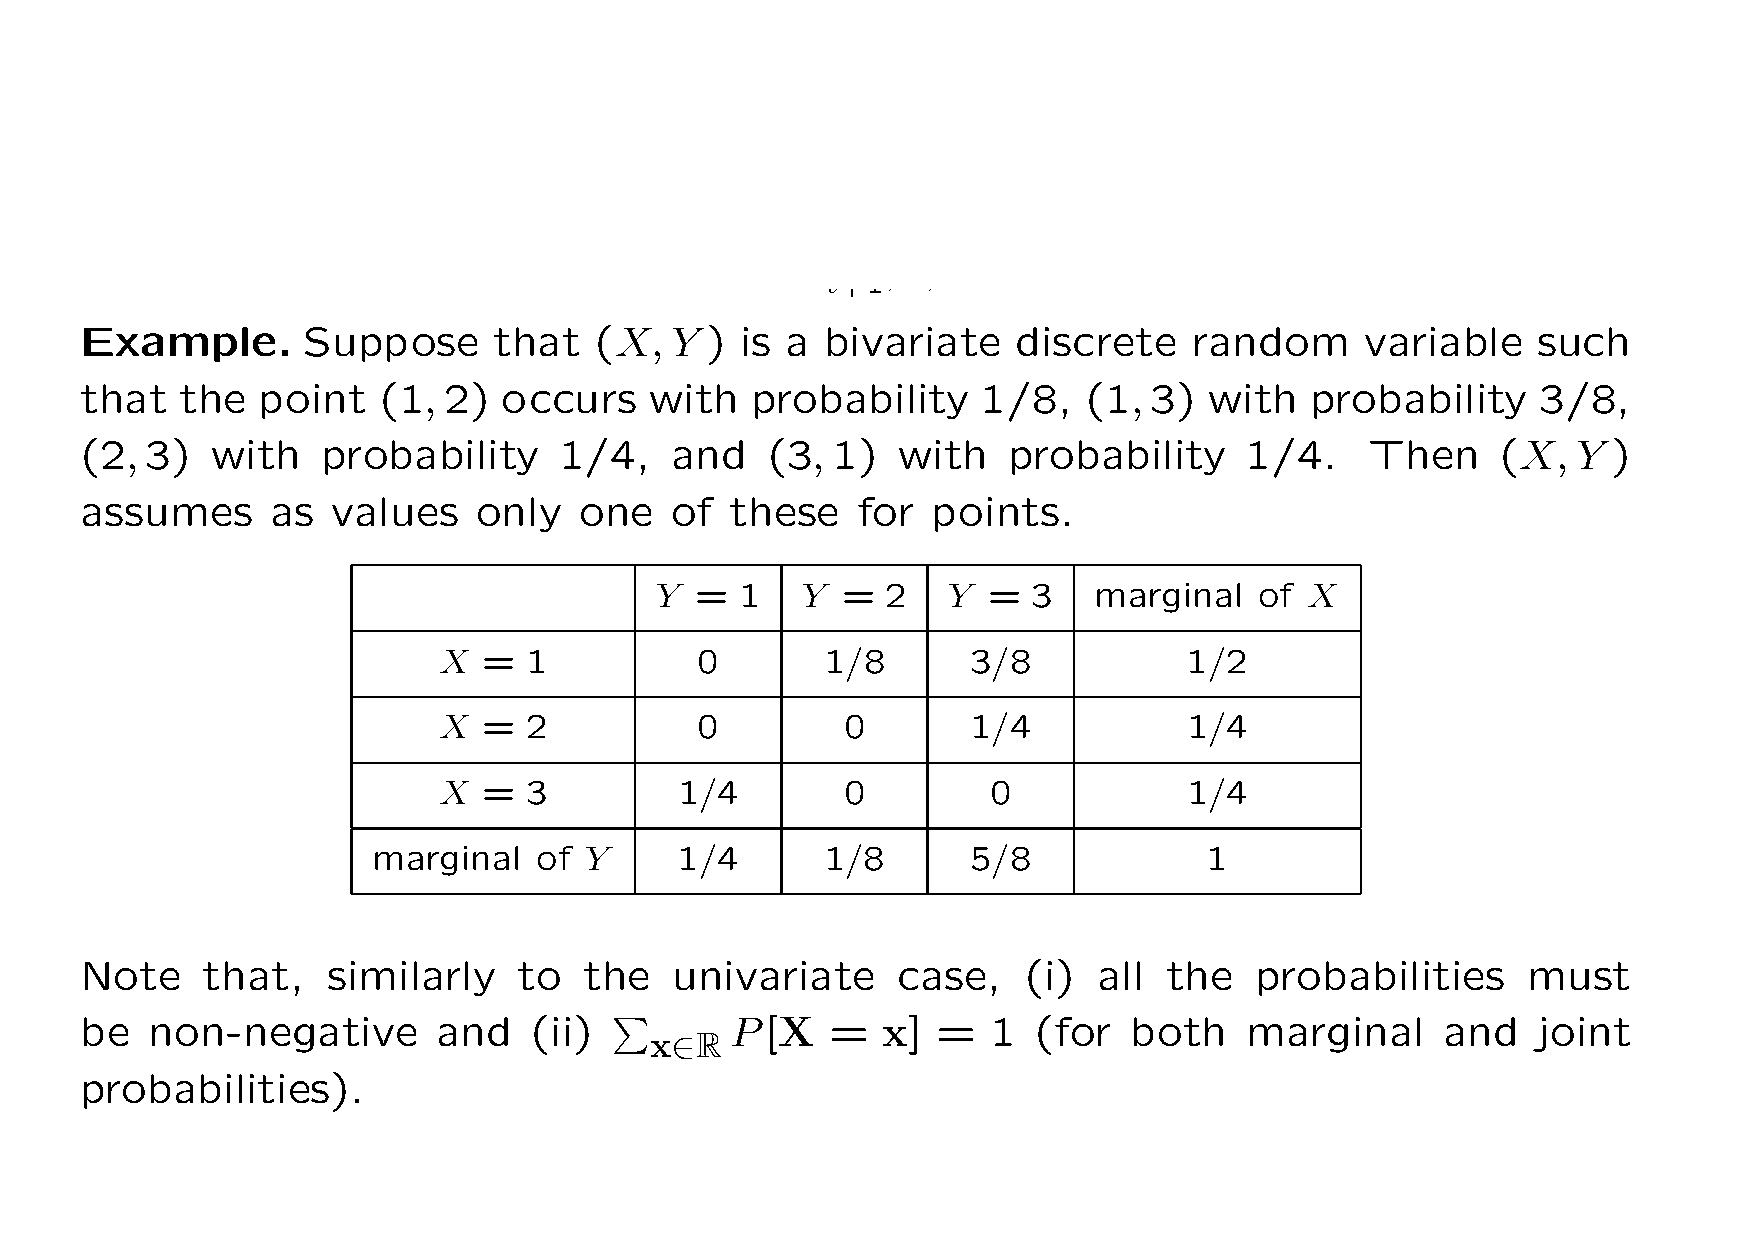
\includegraphics[width=0.95\textwidth,height=0.75\textheight]{img/ex_audrins.pdf}
  \end{figure}
  \end{example}
\end{frame}



\begin{frame}{\secname}
  % \framesubtitle{Expectations for Jointly Distributed Discrete RVs}
  \begin{example}
  \begin{figure}[ptb]\centering
  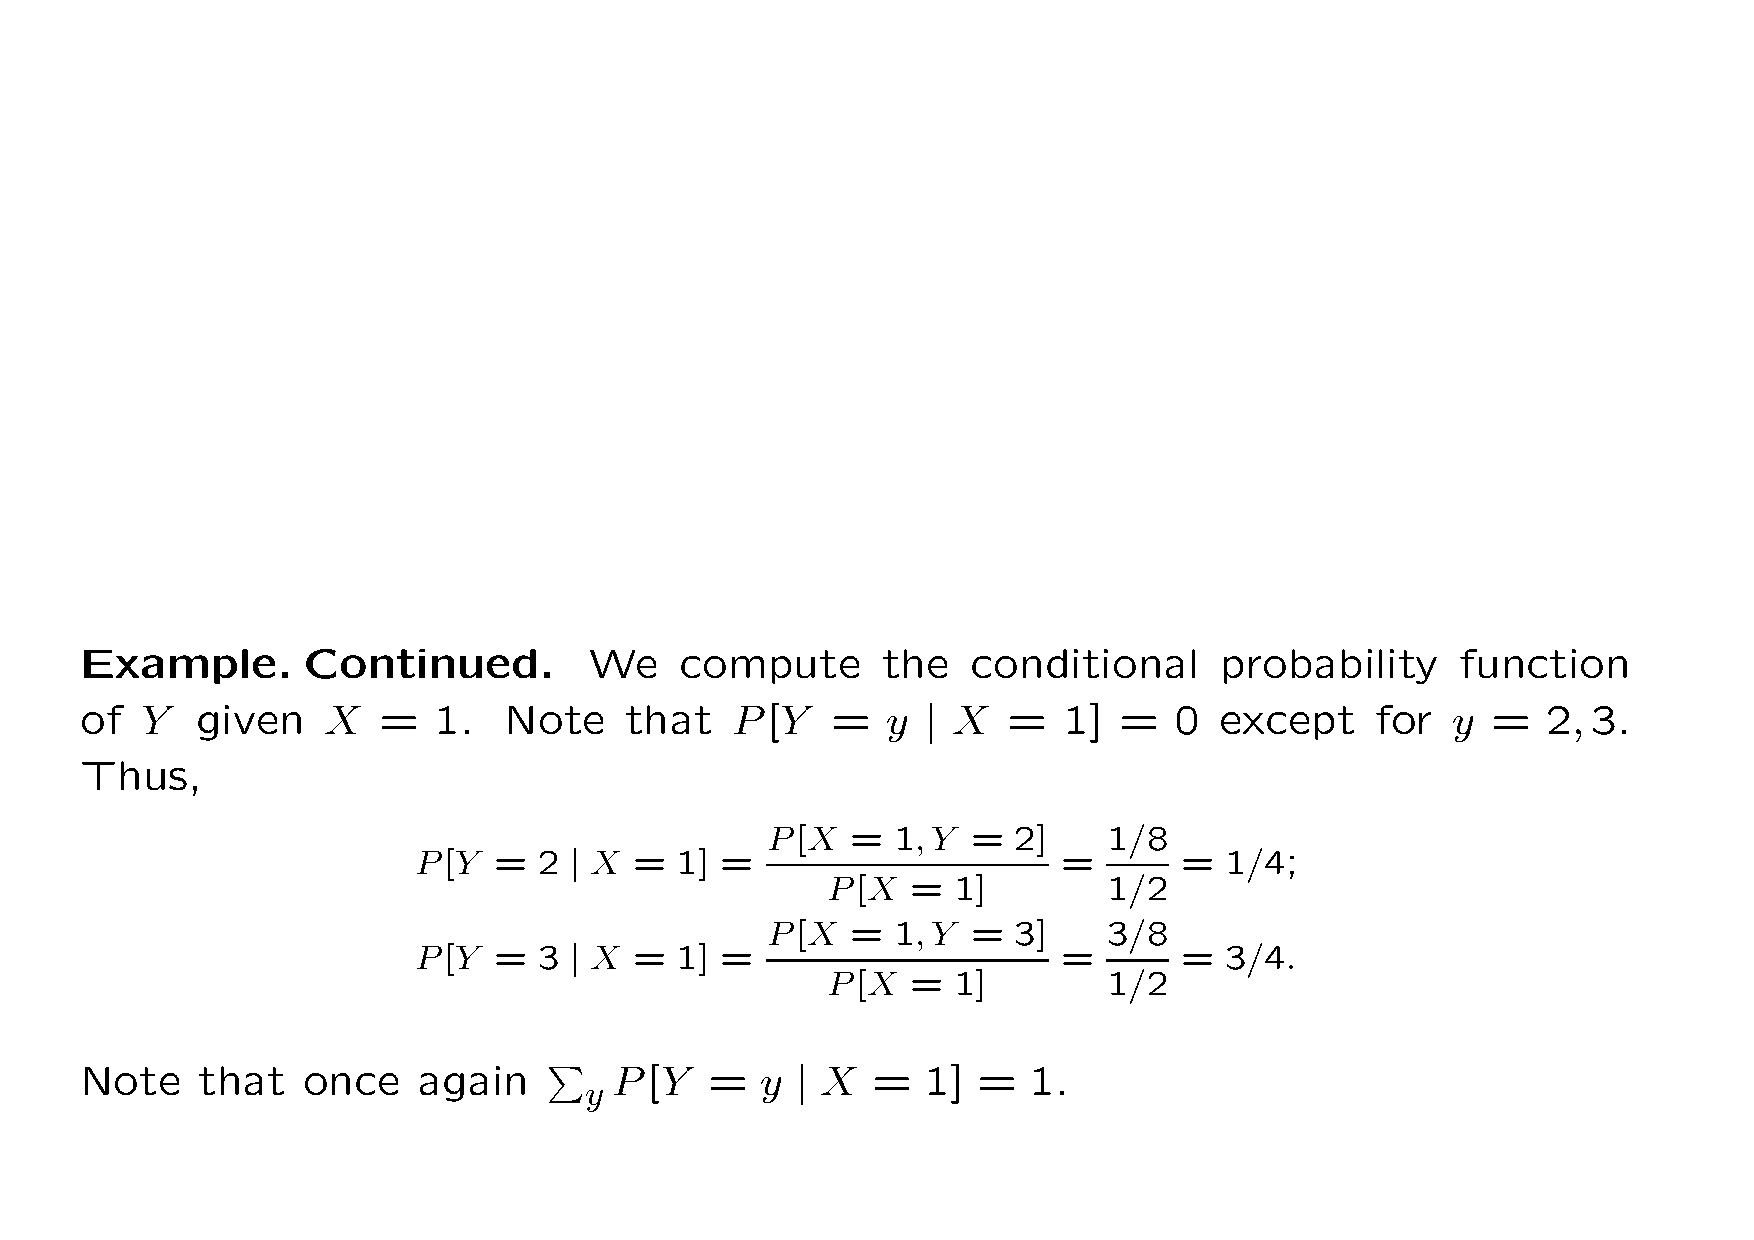
\includegraphics[width=0.9\textwidth,height=0.45\textheight]{img/ex_audrins_2.pdf}
  \end{figure}
  \end{example}
\end{frame}

%%%%%%%%%%%%%%%%%%%%%%%%%%%%%%%%%%%%%%%%%%%%%%%%%%%%%%%%%%%%%%%%%%%%%%%%%%%%%%%%
\section{Expectations}
%%%%%%%%%%%%%%%%%%%%%%%%%%%%%%%%%%%%%%%%%%%%%%%%%%%%%%%%%%%%%%%%%%%%%%%%%%%%%%%%

\begin{frame}{\secname}
\begin{definition}[Expectation of a Function of Two discrete RV]
Let $h(x,y)$ be a function of $x$ and $y$.
We define the \textbf{expected value} of $h\left( X,Y\right) $ as%
\begin{equation*}
E\left[ h\left( X,Y\right) \right] =\sum_{y}\sum_{x}h\left( x,y\right)
p_{X,Y}\left( x,y\right)
\end{equation*}
\end{definition}
\end{frame}%

\begin{frame}{\secname}
  \begin{example}
  \begin{figure}[ptb]\centering
  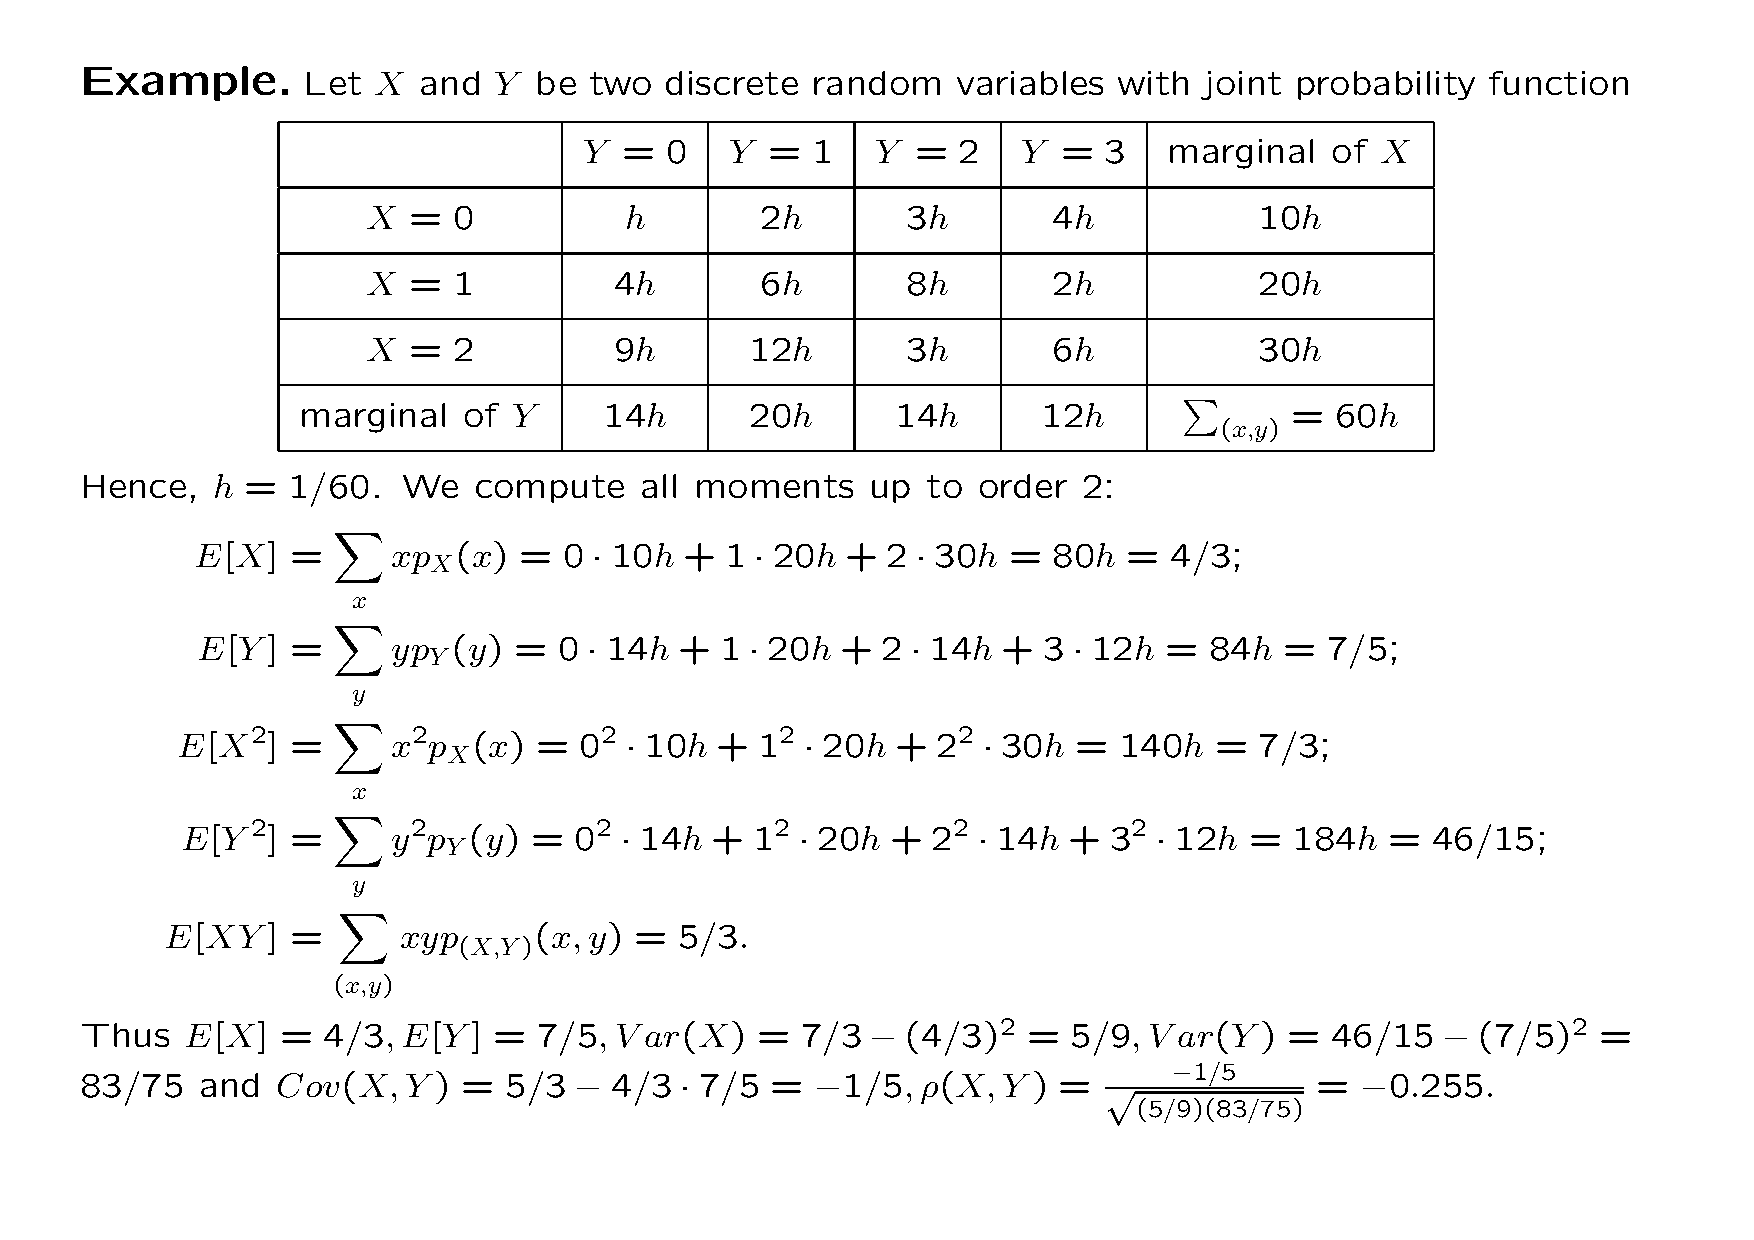
\includegraphics[scale = 0.35]{img/ex_tot.pdf}
  \end{figure}
  \end{example}
\end{frame}

\begin{frame}{\secname}

  \begin{definition}[Conditional Expectation]
  The \textbf{conditional expectation} of $h\left( X,Y\right) $
  \emph{given} $Y=y$ is defined as%
  \begin{equation*}
  E\left[ h\left( X,Y\right) |y\right] =\sum_{x}h\left( x,y\right)
  p_{X|Y}\left( x|y\right).
  \end{equation*}

  \end{definition}
  Equivalently, the \textbf{conditional expectation }of $h\left( X,Y\right) $
  \emph{given} $X=x$ is:
  \begin{equation*}
  E\left[ h\left( X,Y\right) |x\right] =\sum_{y}h\left( x,y\right)
  p_{Y|X}\left( y|x\right).
  \end{equation*}
\end{frame}

\begin{frame}{\secname}
  \begin{example}[continuing the example at page 10]
  \begin{figure}[ptb]\centering
  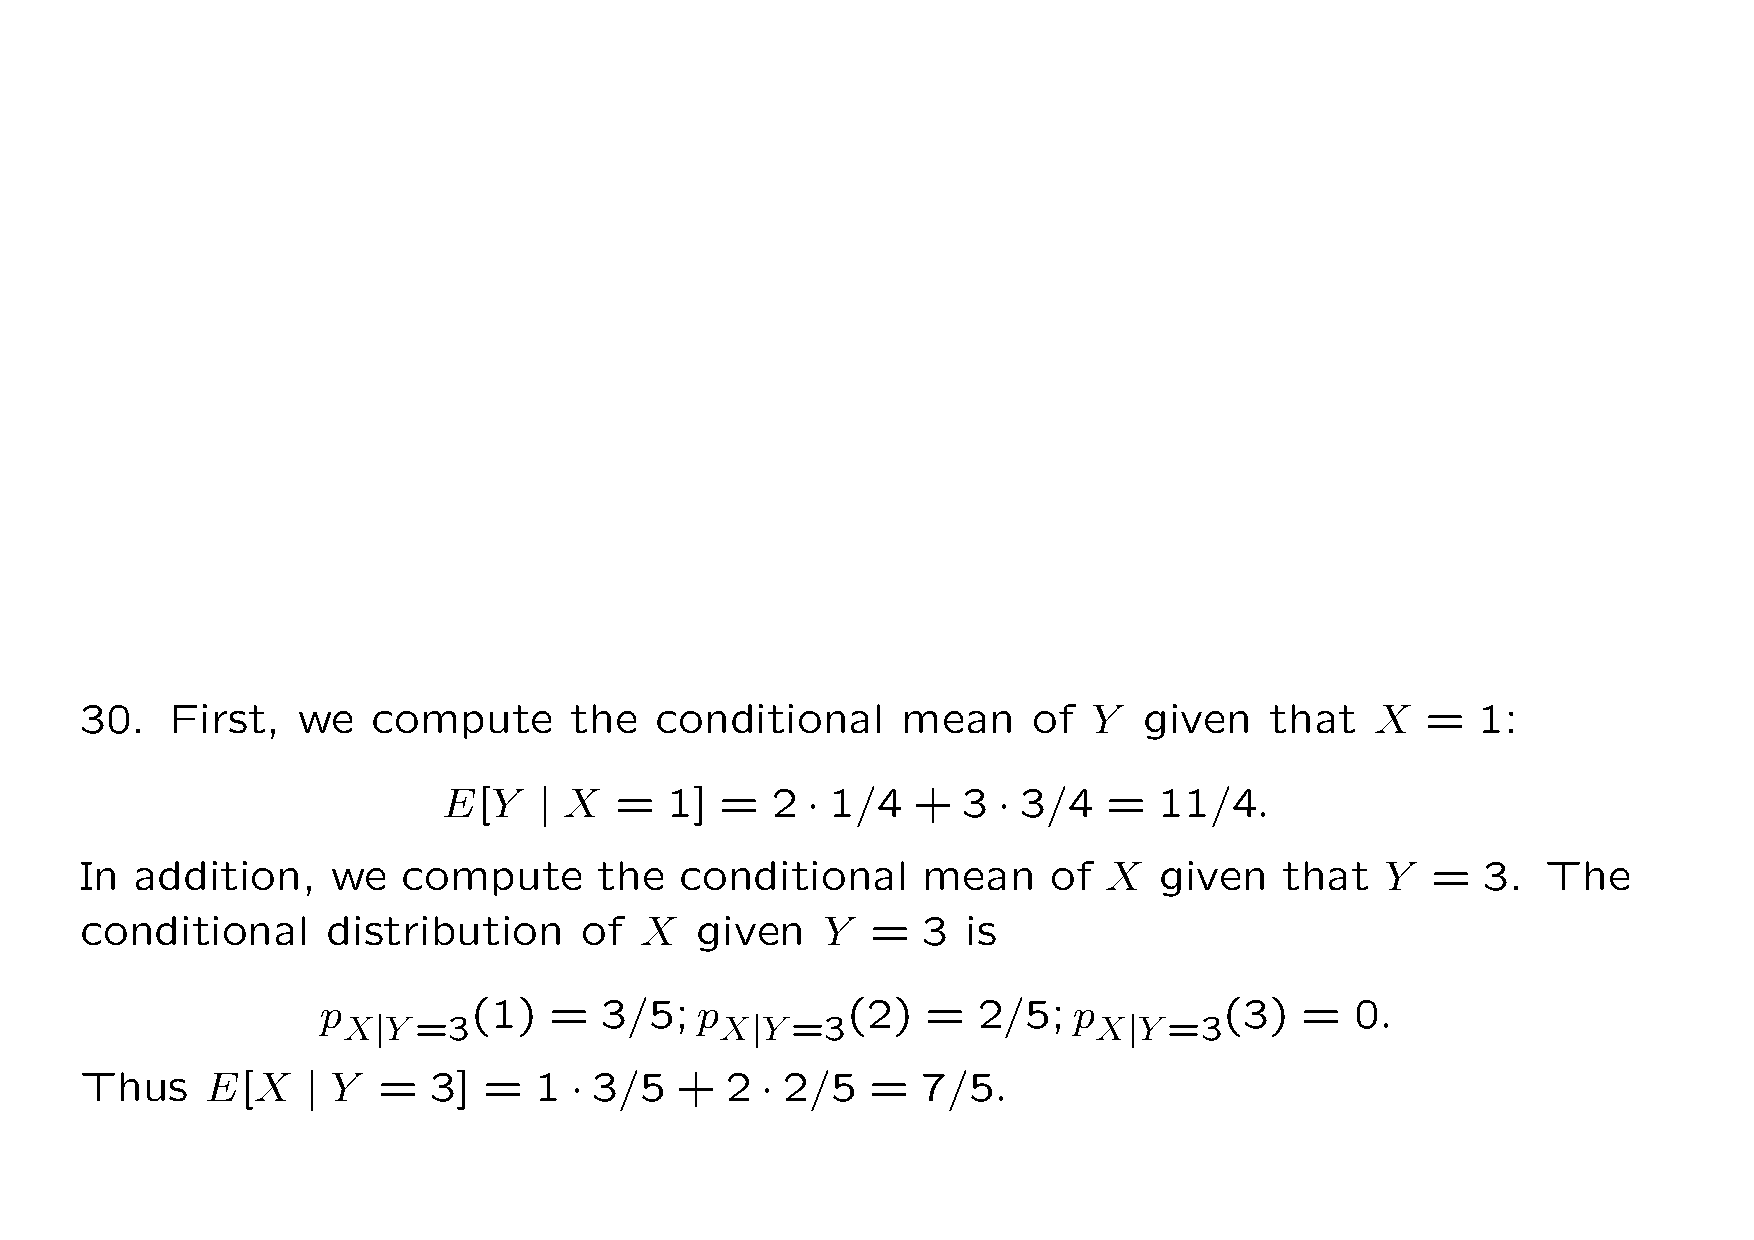
\includegraphics[width=0.9\textwidth,height=0.4\textheight]{img/ex_cond_audrins.pdf}
  \end{figure}
  \end{example}
\end{frame}

%EndExpansion
%
%%TCIMACRO{\TeXButton{BeginFrame}{\begin{frame}{\secname}}}%
%%BeginExpansion
%\begin{frame}{\secname}%
%%EndExpansion
%
%\framesubtitle{Expectations for Jointly Distributed Continuous RVs}
%
%\begin{stepitemize}
%\item Let $h(x,y)$ be a function of $x$ and $y$
%
%\item We define the \textbf{expected value} of $h\left( X,Y\right) $ as%
%\begin{equation*}
%E\left[ h\left( X,Y\right) \right] =\int_{y}\int_{x}h\left( x,y\right)
%f_{X,Y}\left( x,y\right) dxdy
%\end{equation*}
%
%\item Further, the \textbf{conditional expectation }of $h\left( X,Y\right) $
%\emph{given} $Y=y$ is defined as%
%\begin{equation*}
%E\left[ h\left( X,Y\right) |Y=y\right] =\int_{x}h\left( x,y\right)
%f_{X|Y}\left( x|y\right) dx
%\end{equation*}
%
%\item And, the \textbf{conditional expectation }of $h\left( X,Y\right) $
%\emph{given} $X=x$ is defined as%
%\begin{equation*}
%E\left[ h\left( X,Y\right) |X=x\right] =\int_{y}h\left( x,y\right)
%f_{Y|X}\left( y|x\right) dy
%\end{equation*}
%\end{stepitemize}
%
%%TCIMACRO{\TeXButton{EndFrame}{\end{frame}}}%
%%BeginExpansion
%\end{frame}%
%%EndExpansion
%
%%TCIMACRO{\TeXButton{EndFrame}{\end{frame}}}%
%%BeginExpansion
%\end{frame}%
%%EndExpansion
%



\begin{frame}{\secname}%
  \framesubtitle{Iterated Expectations}
  \begin{definition}[Law of the iterated expectation]
  The \textit{law of the iterated expectation} is often stated in the
  form
  \begin{equation*}
  E[h(X,Y)]=E[E[h(X,Y)|Y]]=E[E[h(X,Y)|X]]
  \end{equation*}
  \end{definition}

  \begin{itemize}
    \item This notation emphasises that when we write down $E[\cdot]$ we take the
    expectation with respect to the \textbf{distribution implied by the argument}.
    \item Let's be more explicit:
    \begin{align*}
      E_{(X,Y)}[h(X,Y)] &=E_{Y}\left[E_{X|Y}\left[h(X,Y) \vert Y \right]\right] \\
                        &=E_{X}[E_{Y|X}[h(X,Y) \vert X]].
    \end{align*}
  \end{itemize}
\end{frame}


%%%%%%%%%%%%%%%%%%%%%%%%%%%%%%%%%%%%%%%%%%%%%%%%%%%%%%%%%%%%%%%%%%%%%%%%%%%%%%%%
\section{Covariance and Correlation}
%%%%%%%%%%%%%%%%%%%%%%%%%%%%%%%%%%%%%%%%%%%%%%%%%%%%%%%%%%%%%%%%%%%%%%%%%%%%%%%%

\begin{frame}{\secname}
  \begin{definition}
  Let $X$ and $Y$ be two discrete random variables.
  The \textbf{covariance} between $X$ and\textbf{\ }$Y$ is given by $%
  E\left[ h\left(X,Y\right) \right] $ when%
  \begin{equation*}
  h\left(X,Y\right) =%
  \left(X-E\left[ X\right] \right) \left( Y-E\left[ Y\right] \right),%
  \end{equation*}
  i.e. $Cov\left(X,Y\right) =E\left[ \left(X-E\left[ X\right] \right)
  \left(Y-E\left[ Y\right] \right) \right] $
  \end{definition}

  Alternative formula\footnote{To get it, expand
  $$\left(X-E\left[ X\right] \right) \left( Y-E\left[ Y\right] \right)=XY-E\left[ X\right]Y -XE\left[ Y\right] +E\left[ X\right]E\left[ Y\right]$$ and make use of the properties of expectation.} for $Cov(X,Y)$ is%
  \begin{equation}
  \boxed{Cov\left( X,Y\right) =E\left[ XY\right] -E\left[ X\right] E\left[ Y\right]\ .} \label{Cov}
  \end{equation}
\end{frame}

\begin{frame}{\secname}
  So, to compute the covariance from a table describing the joint behaviour of $X$ and $Y$, you have to:

  \begin{itemize}
  \item compute the joint expectation $E[XY]$---you get it making use of the joint probability; \vspace{0.2cm}
  \item compute $E[X]$ and $E[Y]$---you get using the marginal probability for $X$ and $Y$; \vspace{0.2cm}
  \item combine these expected values as in formula (\ref{Cov}).

  \end{itemize}

  % See example on page 13 for an illustrative computation.
\end{frame}



% \begin{frame}{\secname}%
%
% \framesubtitle{Some Properties of Covariances }
%
%   \begin{stepitemize}
%
%   \item The Cauchy-Schwartz Inequality states
%   $$(E\left[ XY\right])^2\leq E\left[ X^2\right]E\left[ Y^2\right],
%   $$
%   with equality if, and only if, $\Pr(Y=cX)=1$ for some constant $c$.
%
%   \vspace{0.4cm}
%
%   \item Let $h(a)=E[(Y-aX)^2]$ where $a$ is any number. Then
%   $$
%   0\leq h(a)=E[(Y-aX)^2]=E[X^2]a^2-2E[XY]a+E[Y^2]\,.
%   $$
%   This is a quadratic in $a$, and
%   \item[-] if $h(a)>0$ the roots are real and $4(E[XY])^2-4E[X^2]E[Y^2]<0$,
%   \item[-] if $h(a)=0$ for some $a=c$ then $E[(Y-cX)^2]=0$, which implies that $\Pr(Y-cX=0)=1$.
%   \end{stepitemize}
%
% \end{frame}

\begin{frame}{\secname}
  \framesubtitle{Some Properties of Covariances}

  \begin{remark}
   If two random variables are independent, their covariance is equal to zero.
  \medskip
  Note that the converse is not necessarily true, ie. zero covariance between two random variables does not imply that the variables are independent.

  This asymmetry follows because \textbf{the covariance is  a `measure' of linear dependence.}

  \begin{center}
  Independence $\Rightarrow Cov(X,Y)=0$ but $Cov(X,Y)=0\nRightarrow$ independence.
  \end{center}
  \end{remark}
\end{frame}


\begin{frame}{\secname}
  \framesubtitle{Some Properties of Covariances}
  \begin{example}
  \begin{footnotesize}
  Let us consider two discrete random variable $X$ and $Y$, such that
  $$
  P(\{X=0\})=P(\{X=1\})=P(\{X=-1\})=\frac{1}{3},
  $$
  while $Y=0$ if $X\neq 0$ and $Y=1$, if $X=0$. So we have $E[X]=0$ and $XY=0$. This implies
  $$
  Cov(X,Y) = E[XY] -E[X]E[Y] =0,
  $$
  although $X$ and $Y$ are NOT independent: they are related in a nonlinear way.
  \end{footnotesize}
  \end{example}

\end{frame}

\begin{frame}{\secname}
  \framesubtitle{Some Properties of Covariances}

  Building on this remark, we have

  \begin{stepitemize}

  \item
  %TCIMACRO{\TeXButton{black}{\color{black}}}%
  %BeginExpansion
  \color{black}%
  %EndExpansion
  $Cov(X,Y)>0$ if
  \begin{stepitemize}
  \item large values of $X$ tend to be \emph{linearly }associated with large
  values of $Y$
  \item small values of $X$ tend to be \emph{linearly }associated with small
  values of $Y$\bigskip
  \end{stepitemize}
  \item $Cov(X,Y)<0$ if
  \begin{stepitemize}
  \item large values of $X$ tend to be \emph{linearly }associated with
  \underline{small} values of $Y$
  \item small values of $X$ tend to be \emph{linearly }associated with
  \underline{large} values of $Y$\bigskip
  \end{stepitemize}
  \item When $Cov(X,Y)=0$, $X$ and $Y$ are said to be uncorrelated.
  \end{stepitemize}
  %
  %\textbf{GIACOMO DIMOSTRA PROP 4.2 del Ross a tutorial}
\end{frame}

\begin{frame}{\secname}

  \framesubtitle{Some Properties of Covariances}
  \begin{itemize}
  \item  If $X$ and $Y$ are two random variables (either discrete or continuous) with $Cov(X,Y) \neq 0$, then:
  \begin{equation}
  Var(X + Y) =  Var(X) + Var(Y) + 2 Cov(X,Y) \label{FullVar}
  \end{equation}

  \underline{Compare this expression with the formula on Lecture 3-4}, i.e. in the case of independent rv $X$ and $Y$, we have:
  $$
  Var(X + Y) =  Var(X) + Var(Y),
  $$
  which trivially follows from (\ref{FullVar}) - indeed, for independent random variables, $Cov(X,Y)\equiv 0$.

  \item The covariance depends upon the unit of measurement.

  \end{itemize}
\end{frame}


\begin{frame}{\secname}
\framesubtitle{A remark}

\begin{stepitemize}
\item If we scale $X$ and $Y$, the covariance changes: For $a,b>0$%
\begin{equation*}
Cov\left( aX,bY\right) =abCov\left( X,Y\right)
\end{equation*}

Thus, we introduce the\textbf{\ correlation} between $X$ and $Y$ is
\begin{equation*}
corr\left( X,Y\right) =\frac{Cov\left( X,Y\right) }{\sqrt{Var\left( X\right)
Var\left( Y\right) }}
\end{equation*}

which \emph{does not }depend upon the unit of measurement.


\end{stepitemize}


\end{frame}


%
%\begin{stepitemize}
%\item Proof: For $a,b>0$%
%\begin{eqnarray*}
%corr\left( aX,bY\right)  &=&%
%%TCIMACRO{\TeXButton{Pause}{\pause}}%
%%BeginExpansion
%\pause%
%%EndExpansion
%\frac{Cov\left( aX,bY\right) }{\sqrt{Var\left( aX\right) Var\left( bY\right)
%}}\medskip
%%TCIMACRO{\TeXButton{Pause}{\pause} }%
%%BeginExpansion
%\pause
%%EndExpansion
%\\
%&=&\frac{abCov\left( X,Y\right) }{\sqrt{a^{2}Var\left( X\right)
%b^{2}Var\left( Y\right) }}\medskip
%%TCIMACRO{\TeXButton{Pause}{\pause} }%
%%BeginExpansion
%\pause
%%EndExpansion
%\\
%&=&\frac{abCov\left( X,Y\right) }{ab\sqrt{Var\left( X\right) Var\left(
%Y\right) }}\medskip
%%TCIMACRO{\TeXButton{Pause}{\pause} }%
%%BeginExpansion
%\pause
%%EndExpansion
%\\
%&=&Corr\left( X,Y\right) \medskip
%%TCIMACRO{\TeXButton{Pause}{\pause}}%
%%BeginExpansion
%\pause%
%%EndExpansion
%\end{eqnarray*}
%\end{stepitemize}


\begin{frame}{\secname}%

  \framesubtitle{An important property of correlation}
  \begin{remark}
  The Cauchy-Schwartz Inequality implies that
  %Applying the Cauchy-Schwartz Inequality to $U=X-E\left[ X\right]$ and $V=Y-E\left[ Y\right]$ indicates that%
  \begin{equation*}
  -1\leq corr\left( X,Y\right) \leq 1
  \end{equation*}
  \end{remark}

  \vspace{0.4cm}

  The correlation is typically denoted by the Greek letter $\rho$, so we have
  $$
  \rho(X,Y)= corr\left( X,Y\right).
  $$
\end{frame}

\begin{frame}{Wrap-up}
  \begin{itemize}
  \item Two Random Variables can be Jointly distributed \bigskip
  \item This implies Marginal and Conditional Distributions \bigskip
  \item Expectations can also be conditional and can be calculated \bigskip
  \item Covariance and Correlation are measures of \emph{linear} association\bigskip
  \end{itemize}
\end{frame}

\begin{frame}
  \begin{center}
  \Large{Thank You for your Attention!}

  \bigskip
  \pause

  \Large{``See you'' Next Week}
  \end{center}
\end{frame}

\end{document}
